\documentclass{article}
\usepackage[utf8]{inputenc}
	\addtolength{\oddsidemargin}{-.875in}
		\addtolength{\textheight}{0.5in}
\usepackage{graphicx}
\usepackage[table,xcdraw]{xcolor}
\usepackage{amsmath}
\title{CON101 : Post - Silicon Architecture}
\author{Anirudha Kulkarni}
\date{November 2020}
\usepackage{graphics}
\usepackage{hyperref}
\usepackage[export]{adjustbox}
\usepackage[table,xcdraw]{xcolor}
\usepackage[a4paper, total={6in, 8in}]{geometry}
\begin{document}

\maketitle
\section{Introduction}
Silicon has been dominating the transistors since mid 1990s. It has been used extensively since the beginning. Thanks to intel's aggressive research contribution to the field it always has been growing till date.  
    \subsection{Why Silicon is used for making chips?}
        \subsubsection{Cheap and abundant}
        The Silicon is eighth most abundant element. It occurs as oxides of silicon as sand and is second most abundant element in Earth's crust. Its extraction is also relatively easier than semiconductor counterparts.
        \subsubsection{Semiconductor}
        This is one of the major reason to chose silicon as material for transistors. Transistors need to switch on and off when required. Conductors like metal tend to switched on all the times and its difficult to switch them off. On the other hand, insulators tend to remain in off state and difficult to turn on. Semiconductor which has conductivity in between of conductors and insulators works best with lower potential barrier.
        \subsubsection{Precise control}
        Silicon allows to control the number of holes and electrons by the means of doping to a very high level of precision. Silicon can be extracted to a very high purity and controlled by injecting other atoms as required.
        \subsubsection{Room Temperature}
        The intermediate potential barrier of silicon allows it to operate at room temperature without need to apply significant potentials.
    \subsection{Need for Post-silicon - Moore's Law}
    Moore’s law, stated in 1965 and revised in 1975 says that ”The number of transistors on a microchips doubles every two years”. It has been valid since 1975 and continues to hold almost today. But the law is saturating as time is passing. We are currently at 14nm size of a silicon one transistor, which is almost 70 silicon atoms wide taking size of silicon atom as roughly 0.2 nanometers. Going beyond this seems difficult as we get close to the atomic sizes, quantum effects starts to operate. We are no longer dealing with solid entities but with wave nature of those atoms.  \linebreak
    \linebreak
   \begin{center} 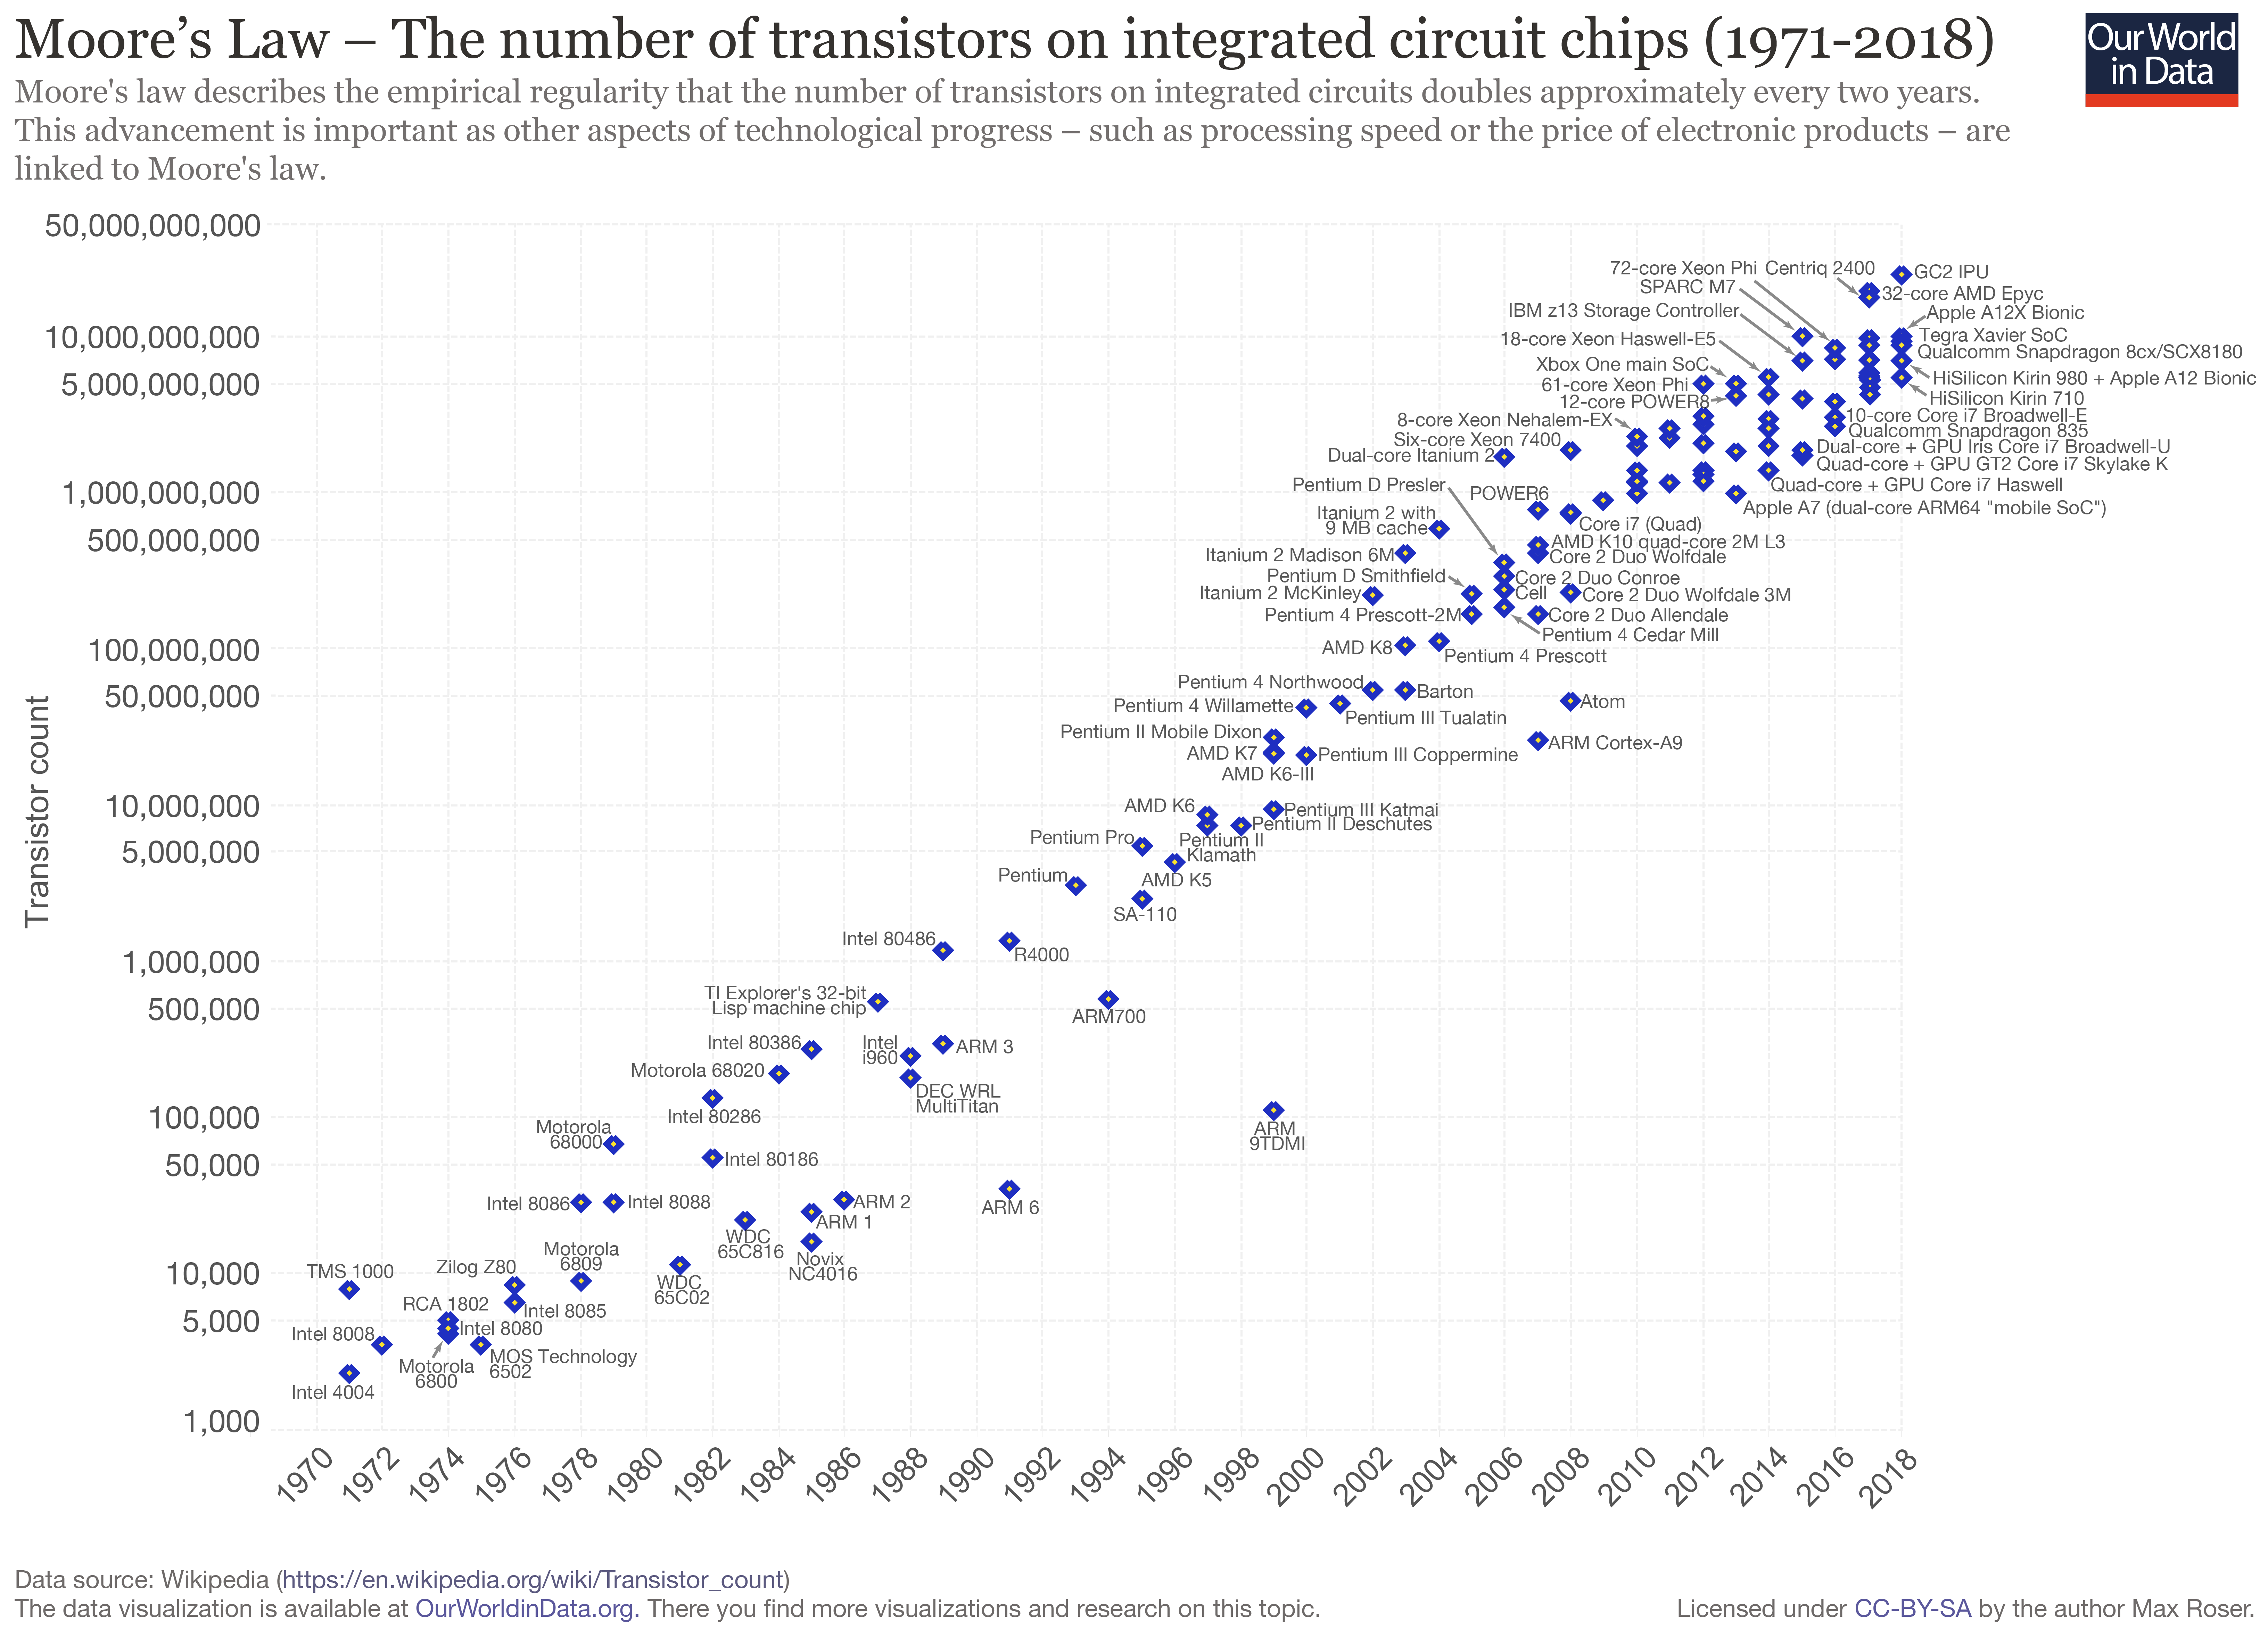
\includegraphics[width=100mm,keepaspectratio]{moore.png}\end{center}
\section{Possible alternatives}
    \subsection{Carbon nanotube / Graphene}
        \subsubsection{What is it?}
        Using carbon allotrope graphene as a substitute to silicon for transistors. Extraordinary electrical properties of cabon nanotubes are from structure of graphene. Graphene based transistors are developed to be single electron transistors i.e. allowing only single electron at a time inside transistor. This is possible due to advancement in carbon nanotubes.
        \subsubsection{Benefits}
        Extremely sensitive and hence can work at relatively lower electron flows. Its faster as speed of electrons travelling between graphene sheets is 1 to 10 thousands time faster than silicon.
        Such transistors can operate at lower voltages compared to silicon. They Require 1/100th amount of power compared to silicon analogue. Due to lower voltages and power consumptions, we can reach higher clock speed without heating issues. This also increases the life of transistors.
        \subsubsection{Challenges}
       Graphene is difficult to prepare as it is much delicate than silicon wafers. Manufacturing such a small layer of graphene is more costly compared to silicons. The technology needed is also still under development. We are yet to reach the stage to use them as sustainable products.
    \subsection{Quantum Computing}
        It simply uses quantum mechanics to perform operations. They hold the potential to increase the computational power exponentially.Quantum computers perform the calculations using the probability of the state of an object. Rather than classical 0 and 1 bits, it works on intermediate states of 0s and 1s too. This unique property is called superposition. The bits are called qubits. The core of quantum computing is Quantum entanglement. Two entangled qubits affect each other from a distance without any direct connection.
        \subsubsection{Benefits}
        Apart from the exponential increase in computational power, we can use quantum computers for modelling many complex situations, molecules, models which are not achievable through classical computers. 
        \subsubsection{Challenges}
        Not all algorithms work efficiently on quantum computers. There is a lot of scope of research on these algorithms so as to make quantum computing more effective and practical. Also, a major issue is with high manufacturing costs and maintenance cost associated with high precision and lower temperatures needed to operate quantum computers.
    \subsection{Optical Computing}
        \subsubsection{What is it?}
        Optical computing is based on using photons ass substitute for electrons. Also, photons have higher bandwidth compared to electrons. Optical storage devices and optical data transfer networks are in everyday use as CDs and optical fibres. But optical transistors are a major part of the computation. Optical transistors are achieved using materials with the non-linear refractive index for creating transistors which allow controlled flow of photons as compared to equivalence in the flow of electrons.
        \subsubsection{Benefits}
        Benefits Photons exceeds the speed of electrons, and hence it results in an increase in computational power.Also, due to lower frictions with medium and other particles, photons are much faster and power efficient. They also reduce the effort needed for coupling with LEDs for transmission via optical fibres.
        \subsubsection{Challenges}
        Optical transmission is effective in long-distance information transmission. But in case of localized computers, they are larger to handle. The high manufacturing cost associated is also a potential barrier. Further long term data reliability is yet to be proven. We might result in loss of data in order to get more computational power
        \pagebreak
\section{Conclusion}
Moore’s law is near to its saturation, and hence there is dire need to shift to non-traditional ways of computing. Apart from the above substitutions, there are other options available such as transistors with three alternative semiconductors such as Gallium nitride, Gallium, Silicon carbide etc., transistors which use nanomagnets to transmit and compute data. Finally coupling photon-based transistors with Quantum computing also has huge potential in the near future. 
\end{document}